%% LyX 2.3.3 created this file.  For more info, see http://www.lyx.org/.
%% Do not edit unless you really know what you are doing.
\documentclass[english]{beamer}
\usepackage{lmodern}
\renewcommand{\sfdefault}{lmss}
\renewcommand{\ttdefault}{lmtt}
\usepackage[T1]{fontenc}
\usepackage{mathtools}
\usepackage{amsmath}
\usepackage{amssymb}
\usepackage{graphicx}

\makeatletter
%%%%%%%%%%%%%%%%%%%%%%%%%%%%%% Textclass specific LaTeX commands.
% this default might be overridden by plain title style
\newcommand\makebeamertitle{\frame{\maketitle}}%
% (ERT) argument for the TOC
\AtBeginDocument{%
  \let\origtableofcontents=\tableofcontents
  \def\tableofcontents{\@ifnextchar[{\origtableofcontents}{\gobbletableofcontents}}
  \def\gobbletableofcontents#1{\origtableofcontents}
}

%%%%%%%%%%%%%%%%%%%%%%%%%%%%%% User specified LaTeX commands.
\usetheme{Warsaw}
% or ...

\setbeamercovered{transparent}
% or whatever (possibly just delete it)

\makeatother

\usepackage{babel}
\begin{document}
\title{Circular Coordinates under Different Cost Functions}
\subtitle{Group 8 Project}
\institute{ICERM August 2019}
\date{Applied Mathematical Modeling with Topological Techniques}
\makebeamertitle
\begin{frame}{Problem Setup}
\begin{itemize}
\item We have a (simplicial) complex $K$ from the dataset $X$, we can
consider the homology and cohomology with a fixed coefficient field
$\mathbb{K}$.
\item Homology and boundary operator: $\partial:C_{k}(K)\rightarrow C_{k-1}(K)$.
e.g. $\partial[a,b,c]=[a,b]+[b,c]+[c,a]$
\item Cohomology and coboundary operator: $\delta:C^{k}(K)\rightarrow C^{k+1}$.
e.g. $\delta\left[\begin{array}{c}
a\mapsto1\\
b\mapsto0\\
c\mapsto0
\end{array}\right]=-[a,b]^{*}-[a,c]^{*}$ where $[a,b]^{*}=\left[\begin{array}{c}
ab\mapsto1\\
bc\mapsto0\\
ca\mapsto0
\end{array}\right]$.
\item Intuition: If you think of boundary operators as ``derivation'',
then the coboundary operator is like ``anti-derivation''.
\item Theorem (Circular Coordinates): Given a $[f]\in H^{1}(K)$, $f$ can
be made into a function $X\rightarrow S^{1}$. This \textbf{circular
coordinate} can be found through the optimization problem $\min_{z\in C^{0}(X)}\|f-\delta z\|_{L^{2}}$.\\
%
\end{itemize}
\begin{itemize}
\item Problem (New): How about we change the cost function $\|x\|_{L^{2}}\coloneqq(\sum_{i}x_{i}^{2})^{1/2}$
into:
\begin{itemize}
\item $\|x\|_{L^{1}}\coloneqq(\sum_{i}|x_{i}|)$ L1-norm\\
It may introduce sparsity across coordinates instead of smoothness.
\item $(1-\lambda)\|x\|_{L^{1}}+\lambda\|x\|_{L^{2}}$ elastic net\\
It may find a balance between L1 and L2 norms.
\item $\|x\|_{L^{1}}+\lambda\|x\|_{L^{p}}$\\
It may produces some other kind of smoothness.
\item Localized penalty. Only take a penalty norm for some subvector of
$x$.
\item In addition, we can penalized not only $x=f-\delta z$ but also
\begin{itemize}
\item $x=\delta z$ (minimize edits?)
\item $x=z$ or $x=z\text{ mod }1$ (smaller values for functions as $X\rightarrow S^{1}$?)
\end{itemize}
\end{itemize}
\end{itemize}
\end{frame}
%
\begin{frame}{Optimization Problem: Gradient Descent}
\begin{itemize}
\item Generic matrix optimization without Jacobian estimate: Slow and inefficient.
\item Matrix optimization using Gradient Descent with Jacobian.
\begin{itemize}
\item Example 1: Annulus.\\
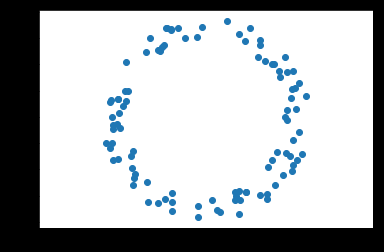
\includegraphics[scale=0.2]{pasted3}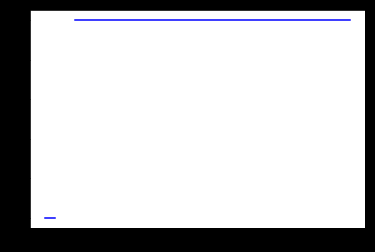
\includegraphics[scale=0.2]{pasted2}
\begin{itemize}
\item L2 norm ($x=f-\delta z$ and $x=z\text{ mod }1$)\\
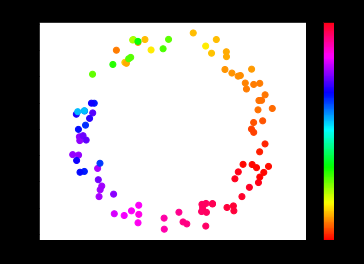
\includegraphics[scale=0.2]{pasted4}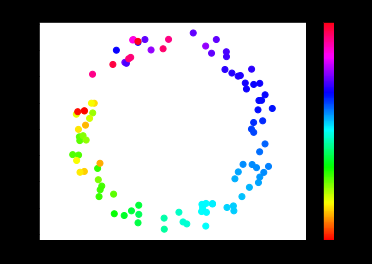
\includegraphics[scale=0.2]{pasted5}
\item L1 norm ($x=f-\delta z$ and $x=z\text{ mod }1$)\\
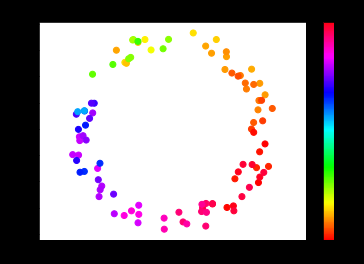
\includegraphics[scale=0.2]{pasted6}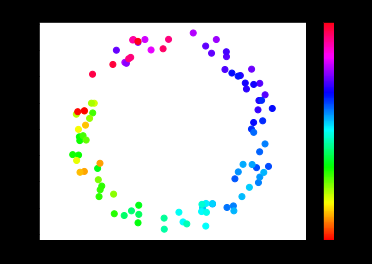
\includegraphics[scale=0.2]{pasted7}\\
\end{itemize}
\end{itemize}
\end{itemize}
\end{frame}
%
\begin{frame}{Another Example}
\begin{itemize}
\item Matrix optimization using Gradient Descent with Jacobian.
\item Example 2: Double Annulus.\\
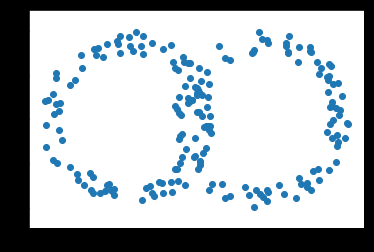
\includegraphics[scale=0.2]{pasted8}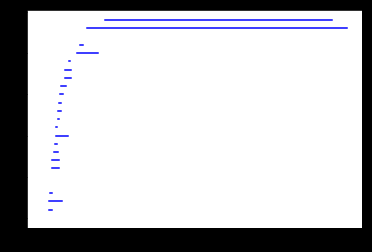
\includegraphics[scale=0.2]{pasted9}
\begin{itemize}
\item Mixed L2 norm ($\|f-\delta z\|_{L^{2}}+||\delta z\|_{L^{2}}$)\\
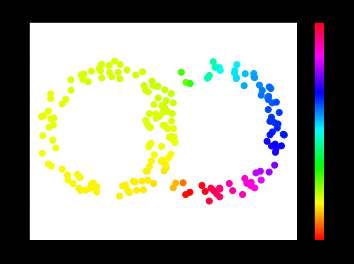
\includegraphics[scale=0.35]{pasted10}
\end{itemize}
\end{itemize}
\end{frame}

\end{document}
